Roll-decay model tests are normally performed prior to other dynamic tests, such as manoeuvring or seakeeping model tests, to check the properties of the tested ship model. In this study, results from such tests, carried out at SSPA in Sweden (www.sspa.se) have been used. The roll-decay tests are conducted by forcing the model to an initial roll angle and then releasing it to oscillate freely in six degrees of freedom. The tests are conducted either  at zero speed or at speed without autopilot. The scaled ship models are from 3 to 6 meters in  length. The measurement accuracy of these model tests is very good. When time series from 20 sets of repeated tests were investigated the average $R^2$ was found to be 0.995. The tests were originally conducted in connection with commercial projects for buildings new merchant ships. In this study, data collected from 2005 to 2018 were used to construct the roll-decay test database, which was applied to build a roll damping database. The ship types in the roll-decay tests used in this paper are  shown in Fig.\ref{fig:ship_types}, and the main parameters of these ships are presented in the sensitivity study as in Fig.\ref{fig:SI_sensitivity}. 
The parameter identification technique was used to estimate the roll damping coefficients from the roll-decay tests. It was investigated whether the linear model Eq.( \ref{eq:roll_decay_equation_himeno_linear}), quadratic model Eq.(\ref{eq:roll_decay_equation_himeno_quadratic_b}) or cubic model Eq.(\ref{eq:roll_decay_equation_cubic}) was best suited to describe the roll damping in all the tests to formulate the roll damping database. After the parameters were identified, the corresponding roll motions were simulated by the three mentioned models. The accuracy of the three models was evaluated with the $R^2$ score coefficient, based on model test and simulation time series of roll motions.
The average $R^2$ was 0.995 for the cubic model, 0.993 for the quadratic, and 0.986 for the linear model. Fig.\ref{fig:roll_decay} displays a linear, a quadratic and a cubic model fitted to one roll decay model test. It is obvious that the linear model, being a straight line in Fig.\ref{fig:roll_decay_damping}, under predicts the damping for large angles and over predicts it for small angles, as can be seen in Fig.\ref{fig:roll_decay_damping}. Since the quadratic model has almost the same accuracy as the cubic model it was selected to estimate roll damping from all the roll-decay tests in the database. All the extracted roll damping coefficients together with various ship related information will be formulated as the roll damping database for the following analysis.

\begin{figure}[H]
    \centering
    \includegraphics[width=0.5\columnwidth]{figures/ship_types.eps}
    \caption{Number of tests per ship type}
    \label{fig:ship_types}
\end{figure}

\begin{figure}[H]
    \begin{subfigure}[b]{0.45\textwidth}
        \centering
        \includegraphics[]{figures/roll_decay_amplitude.eps}
        \caption{Amplitude decrements}
        \label{fig:roll_decay_amplitude}
    \end{subfigure}
        ~ %add desired spacing between images, e. g. ~, \quad, \qquad, \hfill etc. 
      %(or a blank line to force the subfigure onto a new line)
    \begin{subfigure}[b]{0.45\textwidth}
        \centering
        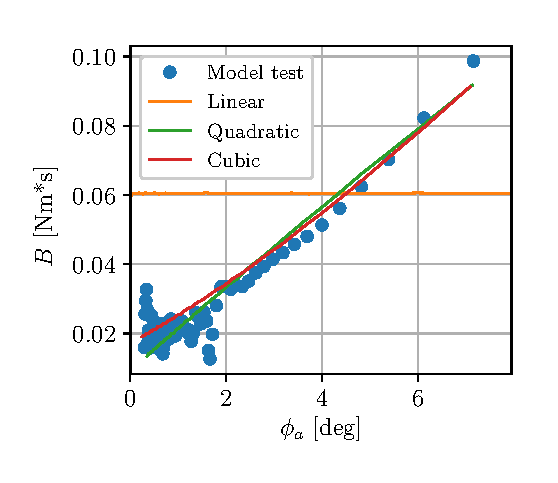
\includegraphics[]{figures/roll_decay_damping.eps}
        \caption{Dampings}
        \label{fig:roll_decay_damping}
    \end{subfigure}
    \caption{Roll decay model test, linear-, quadratic- and cubic-model}
    \label{fig:roll_decay}
\end{figure}


%\begin{figure}[H]
%    \centering
%    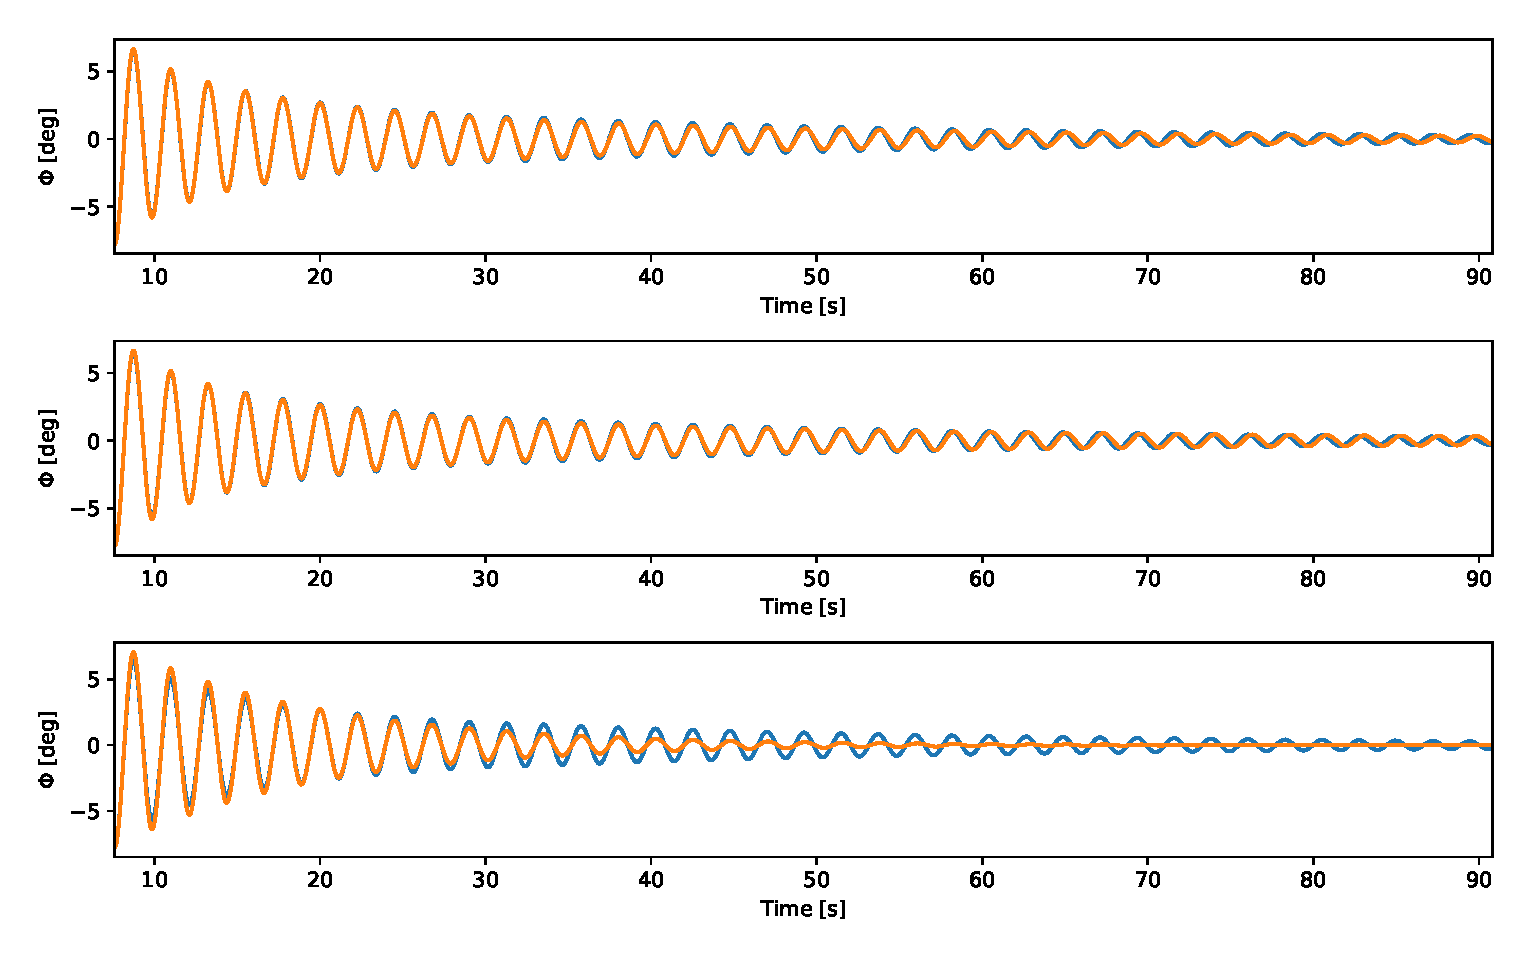
\includegraphics[width=12cm, height = 6cm %]{figures/roll_decay_model_compare.eps}
%        \vspace{-0.5cm}
%    \caption{Roll-decay test comparison of linear (bottom), quadratic %(middle) and cubic model (upper).}
%    \label{fig:roll_decay_model_compare}
%\end{figure}